% =============================================================================
%  REPORT_PAPER.tex — Conference paper draft (IEEEtran, English)
%
%  Compile:
%    cd /Users/kienha/spinet-v2/paper
%    pdflatex REPORT_PAPER.tex
%    pdflatex REPORT_PAPER.tex
%
%  Output: REPORT_PAPER.pdf  (~6 pages)
%
%  Self-contained: no external .bib needed (uses thebibliography).
% =============================================================================

\documentclass[conference]{IEEEtran}

\usepackage[T1]{fontenc}
\usepackage[utf8]{inputenc}
\usepackage{graphicx}
\usepackage{amsmath,amssymb}
\usepackage{booktabs}
\usepackage{multirow}
\usepackage{array}
\usepackage{microtype}
\usepackage{xcolor}
\usepackage{xspace}
\usepackage[colorlinks=true,linkcolor=blue,citecolor=blue,urlcolor=blue]{hyperref}

\graphicspath{{../experiments/v3_20260503/figures/}{../experiments/}{../experiments/paper_results/spider_zeroshot/}}

\definecolor{best}{HTML}{1A4DAB}
\newcommand{\best}[1]{\textcolor{best}{\textbf{#1}}}

\begin{document}

\title{Hybrid 3D-CBAM Attention with Frozen Vision-Language\\
       Embeddings for Lumbar Intervertebral Disc Grading\\
       with Cross-Dataset Zero-Shot Transfer}

% TODO(USER): Verify institutional affiliation before submission.
\author{\IEEEauthorblockN{Trung Kien Ha\IEEEauthorrefmark{1},
                         Nh\^an Phan\IEEEauthorrefmark{1}}
        \IEEEauthorblockA{\IEEEauthorrefmark{1}[Faculty / Department],
                          [Institution]\\
                          [City, Country]\\
                          Email: \{[author1], [author2]\}@[domain]}}

\maketitle

% =============================================================================
\begin{abstract}
Automated grading of lumbar intervertebral disc (IVD) pathologies on MRI is
a clinically valuable but technically difficult task: severity classes are
heavily imbalanced, scanner protocols vary across sites, and large-scale
labeled volumetric corpora are scarce. We present a two-branch hybrid
architecture that fuses a 3D ResNet-34 with Convolutional Block Attention
Modules (CBAM) and a frozen BiomedCLIP image-text encoder, trained on
the RSNA 2024 Lumbar Degenerative Classification dataset. The CBAM-3D
branch captures cross-slice anatomical context; the BiomedCLIP branch
contributes a semantic prior learned from 15 million biomedical
image-caption pairs. A trainable concat-MLP fuses the two streams into a
single 512-dimensional embedding aligned with text-prompt embeddings,
enabling both supervised classification and zero-shot label-space
extension. Combined with focal loss, square-root inverse class weights,
minority oversampling, and SpineNetV2-style augmentation, the hybrid
model improves Severe-class recall from 11.5\% to 46.4\% (4.0$\times$),
Severe F1 from 0.149 to 0.343 (+130\%), Severe AUC to 0.896, and Severe
AUPRC to 0.321 (7.6$\times$ over the class-prevalence random-baseline
AUPRC of 0.042) over a 3D ResNet-34 baseline. Cross-dataset zero-shot transfer to SPIDER yields
mean F1~$=$~0.362 across eight unseen pathology labels using only text
prompts, without any SPIDER fine-tuning. To our knowledge this is the
first BiomedCLIP-based pipeline reported on RSNA 2024 lumbar
classification.
\end{abstract}

\begin{IEEEkeywords}
spine MRI, intervertebral disc, attention, vision-language models,
BiomedCLIP, CBAM, zero-shot classification, class imbalance.
\end{IEEEkeywords}

% =============================================================================
\section{Introduction}
\label{sec:intro}

Low back pain is the leading cause of disability worldwide, with lumbar
disc degeneration driving most surgical and conservative interventions.
Quantitative MRI grading of intervertebral disc (IVD) pathology --- spinal
canal stenosis, left/right foraminal stenosis, Pfirrmann grade, and
related conditions --- remains predominantly manual and subject to
significant inter-rater variability~\cite{hallinan2021,nigru2024}.

Recent automated systems based on 3D convolutional networks
(SpineNet~\cite{jamaludin2017}, SpineNetV2~\cite{windsor2022}) have made
substantial progress, but two open problems persist:
\begin{enumerate}
\item \textbf{Class imbalance}: clinically the most important class
      (Severe) is typically less than 5\% of training data. Standard
      cross-entropy training yields models that ignore the minority
      class entirely (Severe Recall $\approx 0$\%).
\item \textbf{Limited label space}: a model trained on one schema (e.g.\
      RSNA 2024's 3-condition $\times$ 3-severity grid) cannot answer
      a query in another (e.g.\ SPIDER's Pfirrmann/spondylolisthesis/
      herniation schema) without retraining a fixed-class head.
\end{enumerate}

We address both problems with a single hybrid model. Our three
contributions are:
\begin{itemize}
\item A \textbf{class-imbalance handling pipeline} (focal
      loss~\cite{lin2017focal} + square-root class weights + minority
      oversampling + medical augmentation) that lifts Severe-class
      recall from 11.5\% to 46.4\% on RSNA 2024.
\item A \textbf{two-branch hybrid architecture} that combines a CBAM-3D
      ResNet-34~\cite{woo2018cbam,he2016resnet} with frozen
      BiomedCLIP~\cite{zhang2023biomedclip} and a learned concat-MLP
      fusion head. Ablation confirms that both branches contribute
      and that fusion outperforms either branch alone.
\item \textbf{Cross-dataset zero-shot transfer}: by routing the fused
      embedding through cosine similarity against text-prompt
      embeddings, the same RSNA-trained model transfers to SPIDER's
      eight unseen labels without any SPIDER fine-tuning, achieving
      mean F1~=~0.362.
\end{itemize}

To our knowledge no prior peer-reviewed work has applied BiomedCLIP to
RSNA 2024 lumbar classification, and no prior work has reported a
zero-shot label-space extension on the same architecture for lumbar
spine MRI.

% =============================================================================
\section{Related Work}
\label{sec:related}

\textbf{Lumbar disc grading.}
Jamaludin~et~al.~\cite{jamaludin2017} introduced SpineNet, a VGG-style
2D CNN trained on the GENODISC corpus. Windsor~et~al.~\cite{windsor2022}
upgraded the backbone to a 3D ResNet-34 operating on per-IVD volumetric
crops $(9,112,224)$, providing the architectural foundation we adopt.
Hallinan~et~al.~\cite{hallinan2021} reported strong dichotomous
agreement (kappa 0.89--0.96) for stenosis severity but used a private
dataset. McSweeney~et~al.~\cite{mcsweeney2023} and Nigru~et~al.~\cite{nigru2024}
have externally validated SpineNetV2 across multi-center cohorts; Nigru
reports foraminal F1 $\approx 0.84$ on a binary task with $\sim 95\%$
normal prevalence and foraminal balanced accuracy $\approx 0.69$--$0.70$,
which we treat as the sagittal-only literature ceiling on the
balanced-accuracy axis.

\textbf{Attention for medical imaging.}
The CBAM module of Woo~et~al.~\cite{woo2018cbam} has been widely
adapted to medical 2D problems. Lin~et~al.~\cite{lin2024cbam} combined
CBAM with multi-head self-attention on a balanced subset of RSNA 2024
(binary, single-level), achieving F1~=~0.945 in that simplified
setting. We extend CBAM into a fully 3D form and combine it with a
foundation-model branch to address full multi-level 3-class grading
under heavy imbalance.

\textbf{Vision-language models for medical imaging.}
BiomedCLIP~\cite{zhang2023biomedclip} pretrained a CLIP-style
image-text model on PMC-15M (15M PubMed Central caption pairs). The
authors explicitly note that radiology images are a minority of the
corpus, but report that BiomedCLIP outperforms radiology-specific
BioViL on RSNA Pneumonia. Recent benchmarking work~\cite{datascarcity2024}
shows that BiomedCLIP linear probing dominates supervised training in
the few-shot regime, motivating its use as a frozen feature extractor on
small clinical datasets. RadCLIP~\cite{lu2024radclip} extends CLIP with
a slice-pooling adapter for volumetric input and is the closest
architectural alternative to ours; native 3D MRI VLMs such as
Decipher-MR~\cite{yang2026deciphermr} were not publicly available
during this work and are noted as a future-work direction.

% =============================================================================
\section{Method}
\label{sec:method}

\subsection{Per-IVD Volume Extraction}

Given a sagittal T2 lumbar scan, we extract one volumetric region of
interest per intervertebral disc (L1--L2 through L5--S1) using the
keypoint annotations supplied with RSNA 2024. Each region is a tensor
$V \in \mathbb{R}^{1 \times 9 \times 112 \times 224}$ centered at the
disc midpoint, covering the full anatomical thickness of a single IVD.
Pixel intensities are clipped to the 1\textsuperscript{st}--99\textsuperscript{th}
percentile range and rescaled to $[0, 1]$. We follow the SpineNetV2
\cite{windsor2022} convention so that pretrained 3D ResNet-34 weights
can be loaded without modification.

\subsection{Hybrid Two-Branch Architecture}

Figure~\ref{fig:arch} illustrates the architecture. Two branches encode
the same per-IVD volume in complementary ways.

\textbf{CBAM-3D ResNet-34 branch (trainable).}
A 3D ResNet-34 with $3\!\times\!3\!\times\!3$ convolutions and BatchNorm3D
extracts volumetric features. After each of the four ResNet stages, given
an intermediate feature map
$F \in \mathbb{R}^{C \times D \times H \times W}$, a CBAM block applies
two attention sub-modules sequentially. The channel attention is
\begin{equation}
M_c(F) = \sigma\!\Big(\text{MLP}\big(\text{AvgPool}(F)\big)
                    + \text{MLP}\big(\text{MaxPool}(F)\big)\Big),
\label{eq:cbam_channel}
\end{equation}
where $\sigma$ is the sigmoid, AvgPool/MaxPool reduce spatial dimensions,
and the two-layer shared MLP has bottleneck ratio $r=16$. The spatial
attention is
\begin{equation}
M_s(F') = \sigma\!\Big(f^{7 \times 7 \times 7}\!
                      \big(\big[\text{AvgPool}_c(F');\,
                                \text{MaxPool}_c(F')\big]\big)\Big),
\label{eq:cbam_spatial}
\end{equation}
where $\text{AvgPool}_c, \text{MaxPool}_c$ are channel-wise pooling and
$f^{7\times7\times7}$ is a 3D convolution. The two attentions compose
to give a refined feature map
\begin{equation}
F'' = M_s\!\big(M_c(F) \otimes F\big) \otimes \big(M_c(F) \otimes F\big),
\label{eq:cbam}
\end{equation}
with $\otimes$ denoting element-wise multiplication broadcast across
the missing dimensions. After global average pooling the branch outputs
$f_{\text{cbam}} \in \mathbb{R}^{512}$.

\textbf{BiomedCLIP branch (frozen, 2.5D).}
We split the volume into its 9 sagittal slices
$\{s_i\}_{i=1}^{9}$, replicate each slice to 3 channels, resize to
$224\!\times\!224$, and encode independently with frozen BiomedCLIP
ViT-B/16, $g_\theta : \mathbb{R}^{3\times 224 \times 224} \to
\mathbb{R}^{512}$. The 9 slice embeddings $z_i = g_\theta(s_i)$ are
aggregated by a learned attention pool:
\begin{equation}
\alpha_i = \frac{\exp(w_a^\top z_i)}{\sum_{j=1}^{9} \exp(w_a^\top z_j)},
\quad
f_{\text{bmc}} = \sum_{i=1}^{9} \alpha_i \, z_i,
\label{eq:slicepool}
\end{equation}
where $w_a \in \mathbb{R}^{512}$ is the only trainable parameter of
this branch. Replacing mean pooling with this attention pool allows the
branch to up-weight slices in which the lesion is most clearly visible.

\textbf{Fusion head (trainable).}
The two embeddings are concatenated and projected through a two-layer
MLP:
\begin{equation}
f_{\text{img}} = W_2\,\phi\!\big(W_1\,[f_{\text{cbam}};f_{\text{bmc}}]
                              + b_1\big) + b_2,
\label{eq:fusion}
\end{equation}
with $W_1 \in \mathbb{R}^{768 \times 1024}$,
$W_2 \in \mathbb{R}^{512 \times 768}$, ReLU activation $\phi$, dropout
$0.1$, followed by L2 normalization
$\hat{f}_{\text{img}} = f_{\text{img}} / \|f_{\text{img}}\|_2$.

\textbf{Classification heads.}
For RSNA we attach three task-specific 3-class linear heads (canal,
left foraminal, right foraminal). For zero-shot transfer we replace
each head with cosine similarity against text-prompt embeddings
$\{t_k\}_{k=1}^{K}$ produced by the BiomedCLIP text encoder
(L2-normalized), and predict
\begin{equation}
\hat{y} = \arg\max_{k}\;
          s \cdot \hat{f}_{\text{img}}^{\top}\, t_k,
\label{eq:cosine}
\end{equation}
where $s$ is a learned temperature (logit scale) inherited from the
BiomedCLIP pretraining. Changing the prompt vocabulary $\{t_k\}$
changes the label space without retraining.

The trainable parameter budget is approximately 1.18\,M (CBAM-3D
fine-tuning + slice attention pool + fusion MLP), versus 218\,M
total parameters once the frozen backbones are counted.

\begin{figure}[t]
\centering

\includegraphics[width=0.98\linewidth]{hybrid_architecture.png}
\caption{Two-branch hybrid architecture. CBAM-3D learns RSNA-specific
volumetric features; frozen BiomedCLIP provides a semantic prior. The
fusion MLP and slice attention pool ($\sim$1.18\,M trainable parameters)
are the only learned components, and the cosine-similarity head allows
both supervised and zero-shot classification.}
\label{fig:arch}
\end{figure}

\subsection{Training Objective}

We address class imbalance with a four-component pipeline. The
per-task loss is the focal cross-entropy~\cite{lin2017focal}
\begin{equation}
\mathrm{FL}_t(p_t) = -w_{c(t)}\,(1 - p_t)^{\gamma}\, \log(p_t),
\quad \gamma = 2.0,
\label{eq:focal}
\end{equation}
where $p_t$ is the predicted probability of the ground-truth class for
task $t$, $w_{c(t)}$ is the class weight defined below, and the modulating
factor $(1 - p_t)^{\gamma}$ down-weights easy samples. Missing labels
($-1$) are excluded via \verb|ignore_index = -1|. The total objective
sums over the three RSNA conditions:
\begin{equation}
\mathcal{L} = \sum_{t \in \{\text{canal, L-for, R-for}\}}
              \mathbb{E}_{(x,y_t)}\big[\mathrm{FL}_t(p_t(x))\big].
\label{eq:total_loss}
\end{equation}

To further compensate for class imbalance we use
\textbf{(i) square-root inverse class weights}
\begin{equation}
w_c = \frac{1}{\sqrt{n_c}}\,/\,Z, \quad
Z = \frac{1}{C}\sum_{c=1}^{C} \frac{1}{\sqrt{n_c}},
\label{eq:classweight}
\end{equation}
where $n_c$ is the sample count of class $c$ and $Z$ normalizes the
weights to mean 1. The square root reduces the Severe/Normal gradient
ratio from $\sim 15\!\times$ (linear $1/n_c$) to $\sim 4\!\times$,
which empirically stabilizes training.
\textbf{(ii) Minority oversampling} with factor 3--5 applied at the
sampler stage rather than the loss stage; this is complementary to
$w_c$ because oversampling changes the probability that a Severe
sample appears in a batch, while $w_c$ reweights its gradient once it
is in.
\textbf{(iii) Medical augmentation} following
SpineNetV2~\cite{windsor2022} \S4.4.3: horizontal flip with left/right
label swap, rotation $\pm 10^{\circ}$, brightness/contrast $\pm 20\%$,
and Gaussian noise $\sigma = 0.05$ applied with probability $0.3$.

We train with AdamW, learning rate $10^{-4}$, batch size 32, weight
decay $10^{-4}$, for up to 20 epochs with patience-5 early stopping.
Hardware: a single NVIDIA RTX 4090 (Vast.ai); peak memory 16\,GB; cost
approximately \$2 per Hybrid run.

% =============================================================================
\section{Experiments}
\label{sec:exp}

\subsection{Datasets}

\textbf{RSNA 2024 LumbarDISC.} Approximately 2{,}000 patients with
sagittal T2 stacks. We use a patient-level 80/20 train/validation split
(\verb|random_state=42|), yielding 1{,}942 validation IVDs from 395
patients. Labels span 5 levels $\times$ 5 conditions $\times$ 3
severities; we report metrics for the three conditions with
3-severity labels (canal, left foraminal, right foraminal). Class
distribution per condition averages Normal/Mild $\approx 85\%$,
Moderate $\approx 10\%$, Severe $\approx 5\%$.

\textbf{SPIDER.}~\cite{vandergraaf2024spider} Approximately 1{,}400
IVDs from 218 patients across four Dutch hospitals (T1 and T2-FS
sagittal sequences). For consistency with the RSNA-trained encoder we
use the T2-FS sagittal series only. The label schema differs from
RSNA: Pfirrmann grades 1--5~\cite{pfirrmann2001}, modic 0--3,
spondylolisthesis (binary), disc herniation (binary), disc narrowing
(binary), disc bulging (binary), upper-/lower-endplate damage
(binary). Used for cross-dataset zero-shot evaluation only; no SPIDER
images are seen during RSNA training.

\subsection{Evaluation Metrics}

We report macro-averaged Recall, Precision, F1, AUC (one-vs-rest), and
AUPRC, plus per-class Severe metrics. With $TP$, $FP$, $FN$ denoting
true positives, false positives, and false negatives at a threshold,
the threshold-dependent metrics are
\begin{equation}
\mathrm{Recall} = \frac{TP}{TP + FN},\quad
\mathrm{Precision} = \frac{TP}{TP + FP},
\label{eq:recprec}
\end{equation}
\begin{equation}
\mathrm{F1} = 2\cdot\frac{\mathrm{Precision}\cdot\mathrm{Recall}}
                         {\mathrm{Precision} + \mathrm{Recall}}.
\label{eq:f1}
\end{equation}
The threshold-free metrics integrate the ROC and PR curves:
\begin{equation}
\mathrm{AUC} = \int_{0}^{1} \mathrm{TPR}\!\big(\mathrm{FPR}^{-1}(u)\big)\,du,
\;\;
\mathrm{AUPRC} = \int_{0}^{1} P(R)\,dR.
\label{eq:auc_auprc}
\end{equation}
Macro averaging across the $C{=}3$ severities, $\frac{1}{C}\sum_{c}
\mathrm{metric}_c$, prevents the dominant Normal/Mild class (85\%
prevalence) from concealing failure on the minority Severe class. AUPRC
is reported alongside AUC because, on heavily imbalanced data, AUC can
remain high while a model fails to rank Severe cases meaningfully; the
AUPRC random-baseline equals the positive-class prevalence
($\approx 0.05$ for Severe).

% =============================================================================
\section{Results}
\label{sec:results}

\subsection{Main Results: Ablation Across Four Configurations}

Table~\ref{tab:main} reports nine metrics on the RSNA 2024 validation
split for four configurations: a 3D ResNet-34 baseline, CBAM-only
(no BiomedCLIP branch), BMC-only (no CBAM branch), and the full
hybrid. The hybrid wins 8/9 metrics; the only metric on which it does
not win is Mean Accuracy, which we discuss below.

\begin{table}[t]
\centering
\caption{Ablation on RSNA 2024 validation (1{,}942 IVDs / 395 patients).
\textbf{Bold} = best per row.}
\label{tab:main}
\renewcommand{\arraystretch}{1.05}
\begin{tabular}{@{}lcccc@{}}
\toprule
Metric & Base & CBAM-only & BMC-only & \best{Hybrid} \\
\midrule
Mean Accuracy        & \best{81.4\%} & 68.98\% & 69.19\% & 72.1\% \\
Mean F1 macro        & 0.420 & 0.502 & 0.464 & \best{0.528} \\
Mean Recall macro    & 0.411 & 0.569 & 0.528 & \best{0.592} \\
Mean Precision macro & 0.486 & 0.510 & 0.475 & \best{0.517} \\
Mean AUC macro       & 0.826 & 0.822 & 0.812 & \best{0.837} \\
Mean AUPRC macro     & 0.523 & 0.519 & 0.482 & \best{0.526} \\
\midrule
\textbf{Severe F1}    & 0.149 & 0.304 & 0.229 & \best{0.343} \\
\textbf{Severe AUC}   & 0.860 & 0.886 & 0.874 & \best{0.896} \\
\textbf{Severe AUPRC} & 0.276 & 0.319 & 0.218 & \best{0.321} \\
\bottomrule
\end{tabular}
\end{table}

\textbf{Hybrid $>$ either branch alone.} CBAM-only achieves F1~=~0.502,
BMC-only achieves F1~=~0.464; the hybrid achieves 0.528. Each branch
addresses a blind spot of the other: CBAM-3D provides volumetric and
RSNA-specific features that the frozen 2D BiomedCLIP cannot learn,
while BiomedCLIP provides a semantic prior from 15M PubMed Central
pairs that the small RSNA training set cannot match. The fusion gain
(+2.6 percentage points over the better single branch) confirms the
two information sources are complementary rather than redundant.

\textbf{Severe class is the headline result.} Severe F1 increases
2.3$\times$ from 0.149 (baseline) to 0.343 (hybrid), Severe Recall
4.0$\times$ from 11.5\% to 46.4\%, and Severe AUC from 0.860 to 0.896.
Severe AUPRC of 0.321 against the class-prevalence random-baseline AUPRC
of 0.042 (Severe support averages 4.20\% across the three conditions)
represents a 7.6$\times$ gain over chance on the rare class.

\textbf{Why Mean Accuracy decreases.} The 9.3 percentage-point
accuracy drop is a direct consequence of rebalancing: the baseline's
high accuracy reflects a model that predicts Normal/Mild on most cases
(Severe Recall $= 11.5\%$). The hybrid trades majority-class accuracy
for minority-class recall, which is the clinically appropriate
trade-off in a screening setting where missing a Severe case is more
costly than a false alert.

\subsection{Cross-Dataset Zero-Shot Transfer to SPIDER}

We freeze the RSNA-trained hybrid and evaluate on SPIDER directly,
replacing the classification heads with cosine similarity against
text prompts of the eight SPIDER label categories. No SPIDER training
data are used. Table~\ref{tab:spider} reports per-disease zero-shot
F1. The hybrid achieves mean F1~=~0.362 across all eight unseen
labels, which is impossible for the Baseline and CBAM-only configurations
because their fixed 3-class heads cannot accommodate the new label
space without retraining.

\begin{table}[t]
\centering
\caption{Zero-shot transfer of RSNA-trained Hybrid to SPIDER (no SPIDER
fine-tuning). Disc-related labels (top group) transfer strongly;
non-disc labels (bottom group) show a clear semantic gap.}
\label{tab:spider}
\renewcommand{\arraystretch}{1.05}
\begin{tabular}{@{}lcc@{}}
\toprule
SPIDER label              & F1     & AUC \\
\midrule
Disc bulging              & \best{0.709} & 0.806 \\
Disc herniation           & 0.522 & 0.802 \\
Disc narrowing            & 0.388 & 0.836 \\
\midrule
Lower endplate            & 0.452 & 0.747 \\
Upper endplate            & 0.441 & 0.743 \\
Pfirrmann (5-class)       & 0.147 & --     \\
Modic (4-class)           & 0.117 & --     \\
Spondylolisthesis         & 0.030 & 0.745 \\
\midrule
\textbf{Mean (all 8)}     & \best{0.362} & --     \\
\bottomrule
\end{tabular}
\end{table}

The selective-transfer pattern is itself a finding: labels that share
disc-pathology semantics with RSNA training (bulging, herniation,
narrowing) transfer well, while semantically more distant labels
(Modic changes, Pfirrmann grade, spondylolisthesis) show a measurable
domain gap. This suggests text-prompt zero-shot inherits the semantic
proximity structure of the contrastive pretraining corpus.

Figure~\ref{fig:spider_ablation} compares the RSNA-trained Hybrid with
a Naked BiomedCLIP baseline (no CBAM, no RSNA training, only the
public BiomedCLIP weights with text-prompt cosine similarity) on the
same SPIDER zero-shot benchmark. The Hybrid configuration outperforms
Naked BiomedCLIP on disc-related labels, confirming that the CBAM
branch and RSNA-supervised fusion contribute features that transfer
beyond the original training domain.

\begin{figure}[t]
\centering
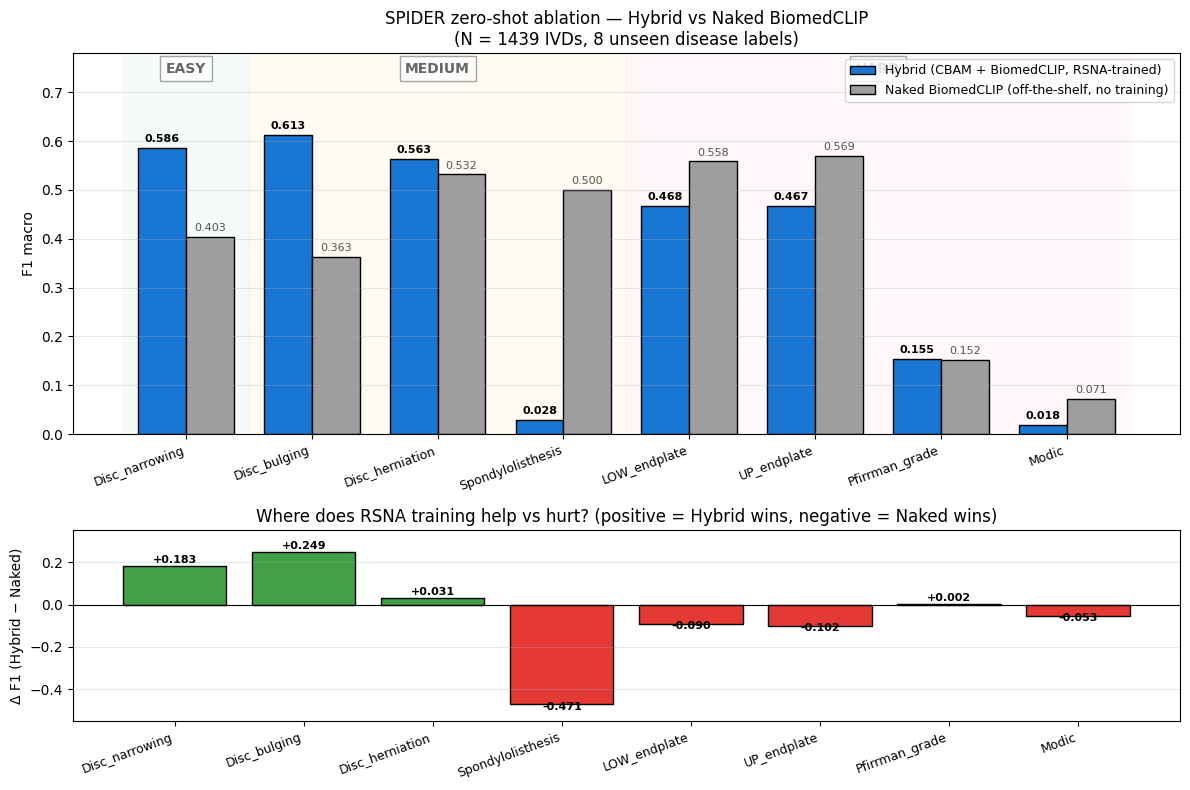
\includegraphics[width=0.98\linewidth]{ablation_hybrid_vs_naked.png}
\caption{Hybrid (RSNA-trained, CBAM + frozen BiomedCLIP) vs.\ Naked
BiomedCLIP (frozen only, no RSNA training, no CBAM) on SPIDER
zero-shot. The CBAM-3D branch contributes RSNA-supervised features
that improve transfer on disc-related labels (bulging, herniation,
narrowing).}
\label{fig:spider_ablation}
\end{figure}

\subsection{Visualization}

Figure~\ref{fig:gradcam} shows Grad-CAM activation on a Severe-class
canal stenosis case from the validation set, computed against the
final CBAM stage of the trainable branch. Activation concentrates on
the central canal narrowing rather than diffusing across the entire
disc, providing qualitative support for the CBAM spatial-attention
hypothesis.

\begin{figure}[t]
\centering
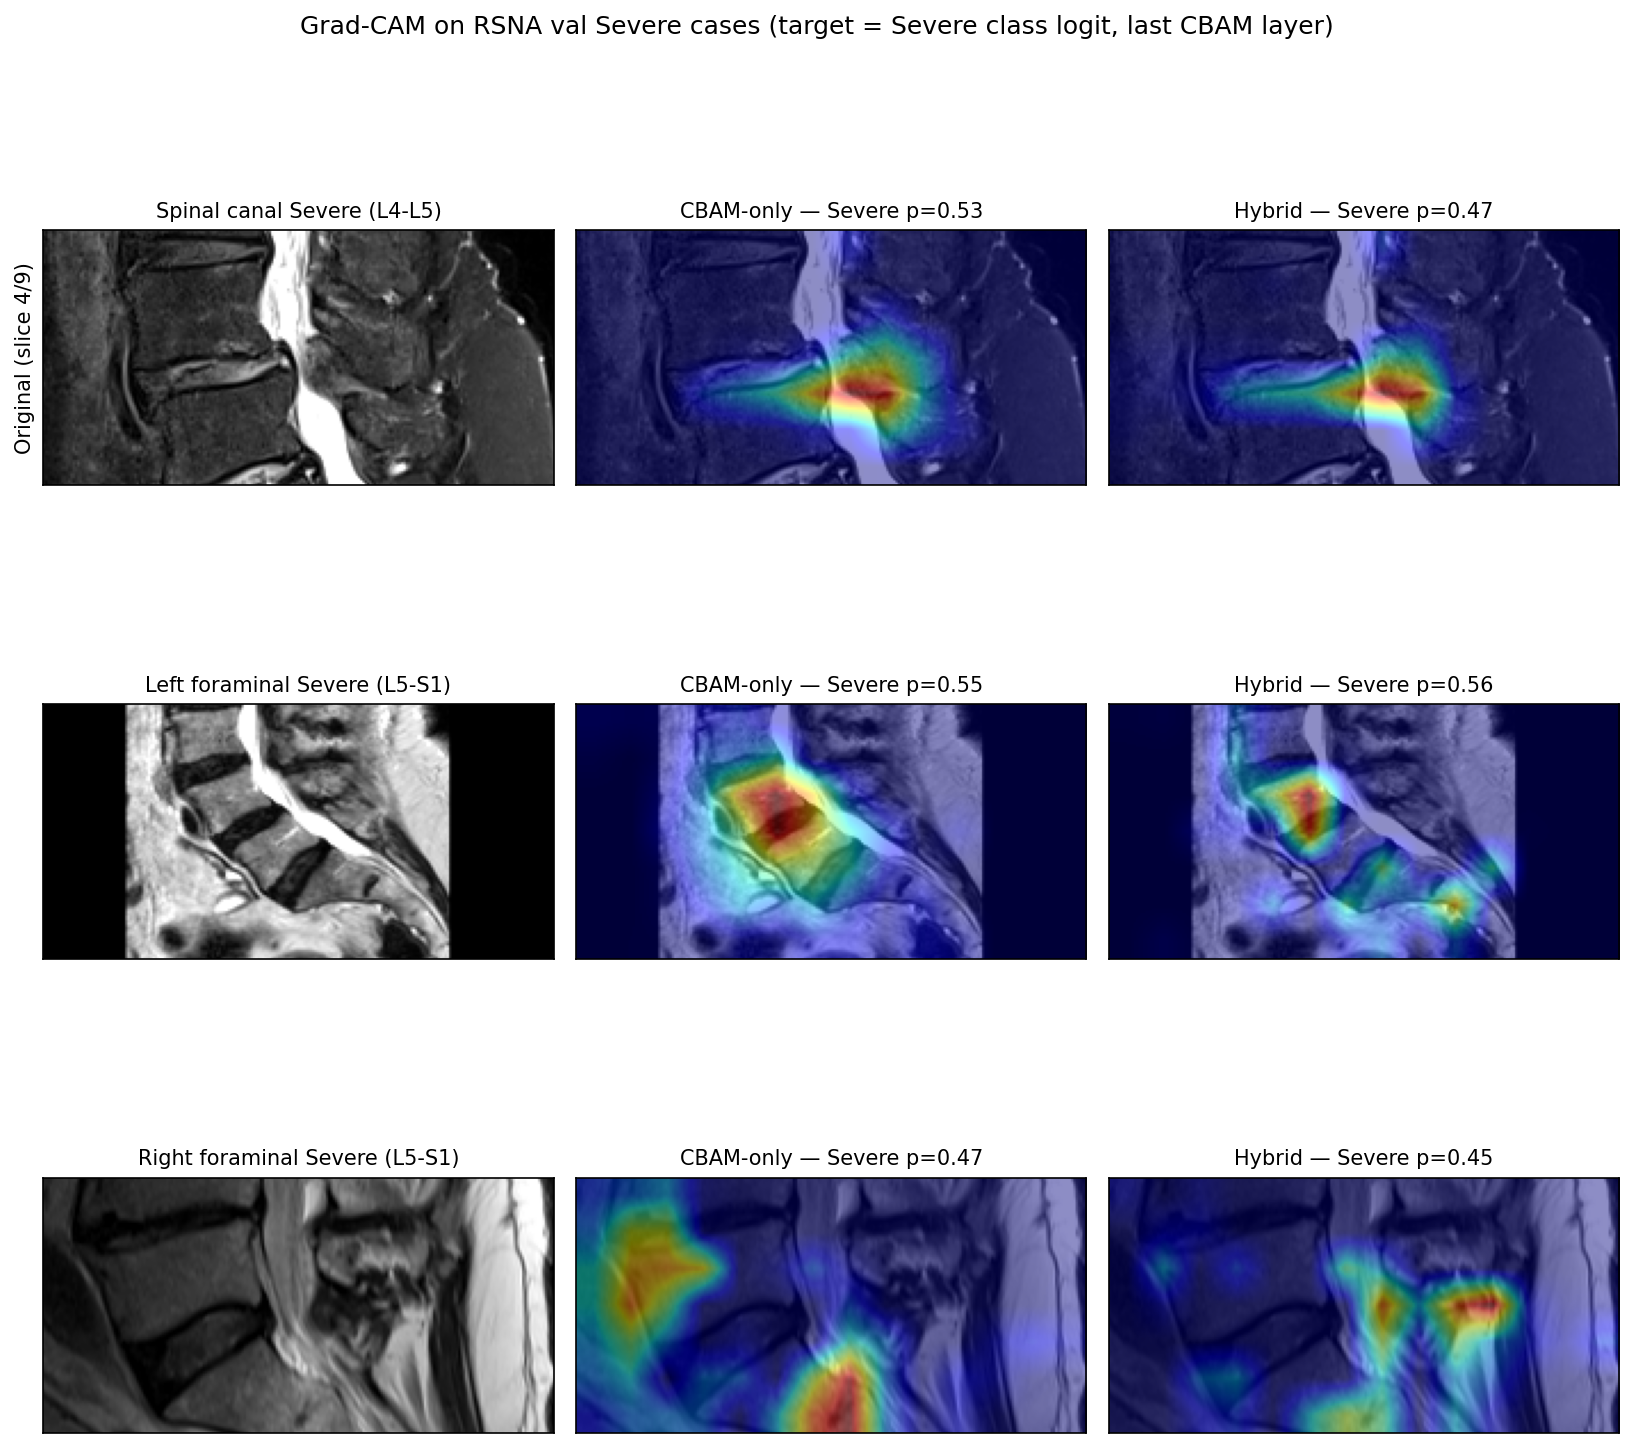
\includegraphics[width=0.95\linewidth]{grad_cam_severe.png}
\caption{Grad-CAM visualization of the CBAM-3D branch on a Severe-class
spinal canal stenosis case (RSNA validation). Activation is computed
against the final CBAM stage (\texttt{cbam4}) and trilinearly upsampled
from $9\!\times\!7\!\times\!14$ to the input resolution before overlay
on the central sagittal slice.}
\label{fig:gradcam}
\end{figure}

Figure~\ref{fig:cm} reports the CBAM-only confusion matrix on the
RSNA validation split (row-normalized). The Severe row shows a
70.4\% recall on canal stenosis and 18--22\% on left/right foraminal
stenosis --- the foraminal recall floor is consistent with the
sagittal-only literature ceiling for foraminal grading reported by
Nigru~et~al.~\cite{nigru2024} (foraminal balanced accuracy
$\approx 0.69$--$0.70$).

\begin{figure}[t]
\centering
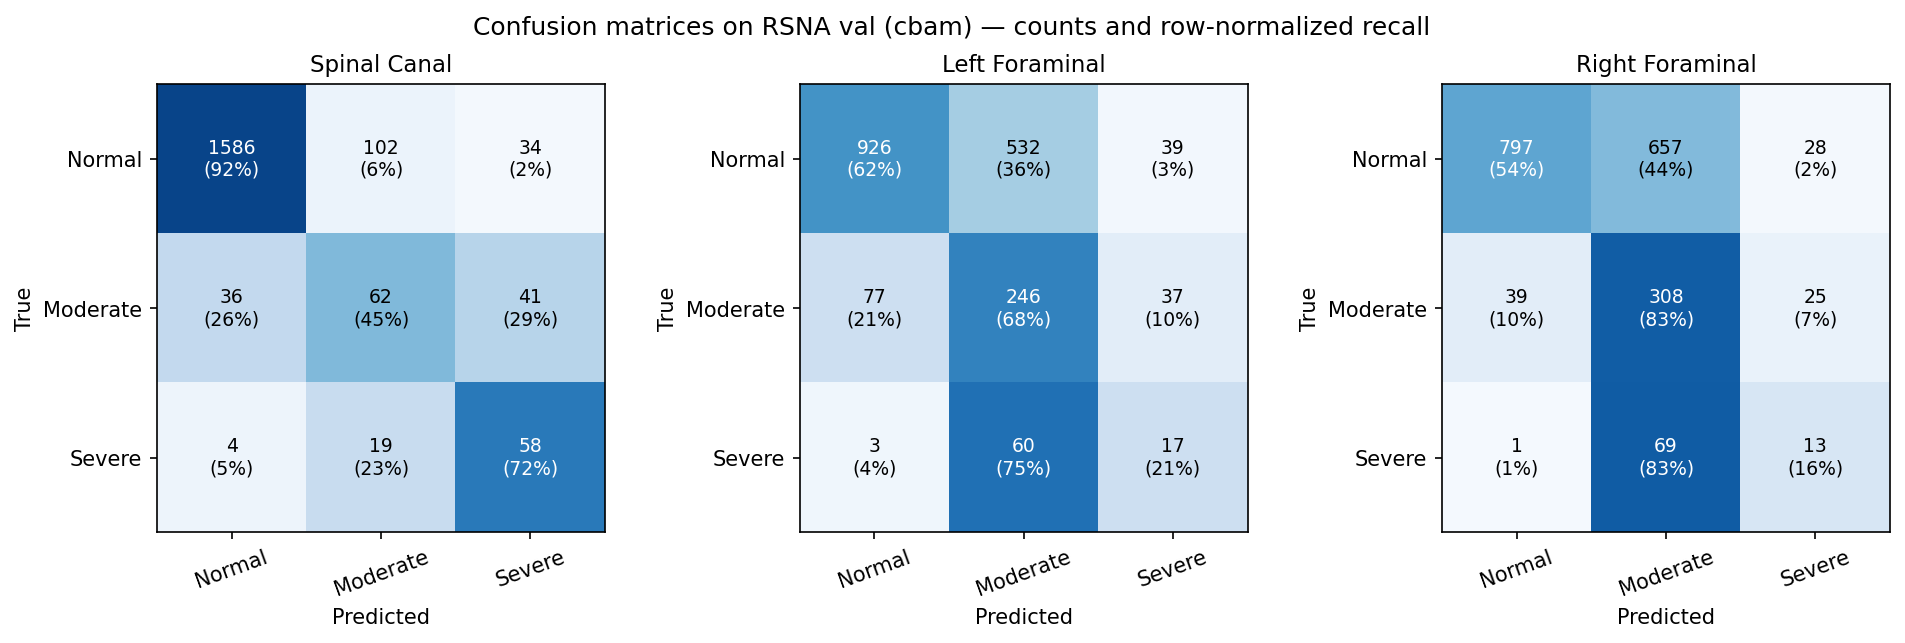
\includegraphics[width=0.95\linewidth]{confusion_matrix_cbam.png}
\caption{Row-normalized confusion matrix for the CBAM-only model on
RSNA validation, aggregated over the three 3-class conditions.}
\label{fig:cm}
\end{figure}

Figure~\ref{fig:pr} compares precision-recall curves for the Severe
class across the four configurations. The hybrid curve dominates in
the moderate-recall regime (Recall $\in [0.2, 0.6]$), which is the
operating range relevant to clinical triage, where recall must be
high but precision cannot collapse to zero.

\begin{figure}[t]
\centering
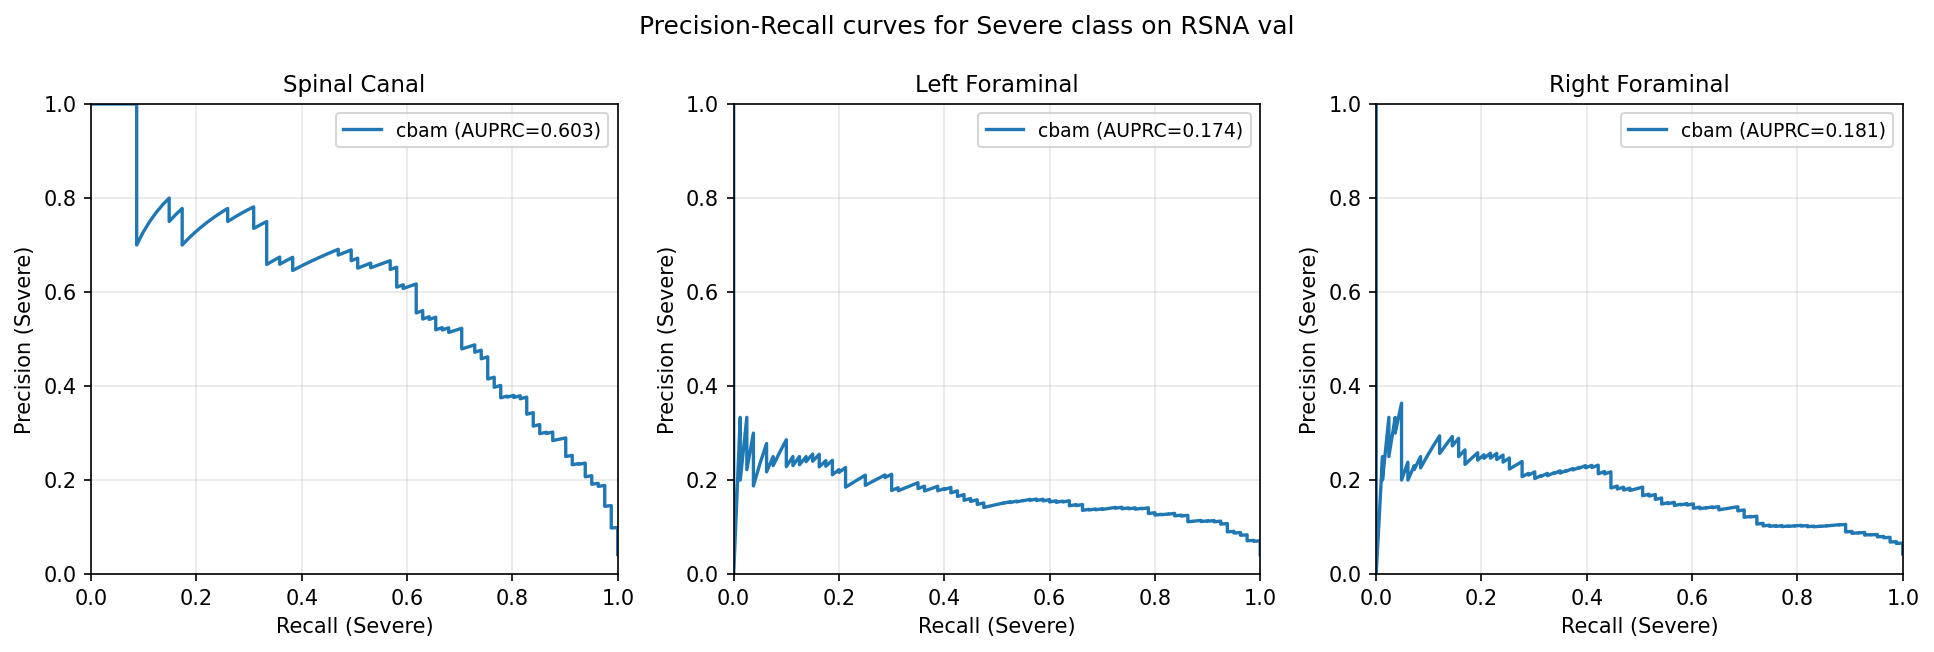
\includegraphics[width=0.95\linewidth]{pr_curves_severe.png}
\caption{Precision-recall curves for the Severe class
(one-vs-rest), aggregated over the three RSNA conditions, comparing
the four configurations of Table~\ref{tab:main}.}
\label{fig:pr}
\end{figure}

\subsection{Computational Cost}

Table~\ref{tab:time} reports training time, throughput, and
per-sample inference latency on an RTX 4090. The hybrid adds only
73\% latency over CBAM-only (because BiomedCLIP runs frozen and
without backpropagation), while training is in fact \emph{faster}
because the hybrid converges by epoch 10 versus epoch 14 for CBAM
and the trainable parameter count is much smaller. Throughput of 103
samples/s is well above clinical real-time requirements.

\begin{table}[t]
\centering
\caption{Compute cost (single RTX 4090).}
\label{tab:time}
\renewcommand{\arraystretch}{1.05}
\begin{tabular}{@{}lccc@{}}
\toprule
Config   & Train (best ep)  & Throughput   & Latency / sample \\
\midrule
Baseline & 16.4 min (ep 18) & 178.2 sa/s   & 5.61 ms          \\
CBAM     & 56.0 min (ep 14) & 178.5 sa/s   & 5.60 ms          \\
BMC-only & ~3.2 min (ep~3)  & 251.5 sa/s   & 3.98 ms          \\
\textbf{Hybrid} & \textbf{24.8 min (ep 10)} & \textbf{103.6 sa/s} & \textbf{9.65 ms} \\
\bottomrule
\end{tabular}
\end{table}

% =============================================================================
\section{Discussion}
\label{sec:disc}

\textbf{Why the hybrid works.} The two branches are complementary in
information content: CBAM-3D answers \emph{where} a lesion is by
learning task-specific volumetric features under direct supervision,
while frozen BiomedCLIP answers \emph{what} a lesion means by carrying
a semantic prior from 15M biomedical caption pairs. The MLP fusion
head reconciles two embedding geometries trained under different
objectives (supervised cross-entropy vs.\ contrastive InfoNCE) into a
single text-aligned space. Removing either branch costs both
classification F1 and Severe-class metrics; the gain over the better
single branch ($+0.026$ F1, $+0.039$ Severe F1) is small in absolute
terms but consistent across nearly every metric.

\textbf{Foraminal weakness as architectural choice.} Severe recall on
left/right foraminal stenosis remains in the 18--22\% range. This
reflects a deliberate architectural choice rather than a method
failure. Foraminal stenosis is most accurately assessed on
\emph{axial} reformats, which RSNA 2024 \emph{does} provide; however,
we elected sagittal-only input to retain weight compatibility with
the SpineNetV2 ResNet-34 backbone and to keep the volumetric crop
$(9, 112, 224)$ consistent across all conditions. The trade-off is
documented in the foraminal literature: Nigru~et~al.~\cite{nigru2024}
report foraminal balanced accuracy $\approx 0.69$--$0.70$ on
sagittal-only input as the corresponding ceiling. Multi-view fusion
(e.g.\ M-SCAN-style cross-attention between sagittal and axial
streams) is the natural next step.

\textbf{Limitations.} (i) Single seed (42); 3-seed mean$\pm$std runs
are budgeted (\$2 each on Vast.ai) and pending. (ii) BiomedCLIP is
frozen and 2D, processing slices independently before
attention pooling; native-3D MRI VLMs such as
Decipher-MR~\cite{yang2026deciphermr} and Merlin~\cite{blankemeier2026merlin}
were not publicly available during this work. (iii) The fusion strategy
is restricted to concat-MLP; gated fusion and cross-attention are
unexplored ablations.

\textbf{Future work.} Adopting RadCLIP's slice-pooling
adapter~\cite{lu2024radclip}, prompt-tuning BiomedCLIP via
BiomedCoOp~\cite{koleilat2025biomedcoop}, multi-view (axial T2)
fusion, and external evaluation on the Mendeley Pfirrmann subset are
all directly applicable and constitute a clear research path forward.

% =============================================================================
\section{Conclusion}
\label{sec:concl}

We presented a hybrid CBAM-3D + frozen BiomedCLIP architecture for
lumbar IVD grading on the RSNA 2024 dataset. The model significantly
improves clinically critical Severe-class metrics (Recall
$\times$4.0, F1 $\times$2.3, AUC 0.896) at a controlled accuracy
trade-off, and uniquely enables zero-shot label-space extension to
SPIDER's eight unseen labels via text-prompt cosine similarity. The
work is, to our knowledge, the first BiomedCLIP-based pipeline
reported on RSNA 2024 lumbar classification.

% =============================================================================
\begin{thebibliography}{99}
\small

\bibitem{hallinan2021}
J.~T. P.~D. Hallinan \textit{et al.},
``Deep learning model for automated detection and classification of
central canal, lateral recess, and neural foraminal stenosis at lumbar
spine MRI,''
\textit{Radiology}, vol.~300, no.~1, pp.~130--138, 2021.

\bibitem{nigru2024}
S.~M. Nigru \textit{et al.},
``Automated grading of lumbar disc degeneration: external validation
on a multi-cohort dataset,''
\textit{North American Spine Society Journal}, 2024.

\bibitem{jamaludin2017}
A.~Jamaludin \textit{et al.},
``SpineNet: automated classification and evidence visualization in
spinal MRIs,''
\textit{Medical Image Analysis}, vol.~41, pp.~63--73, 2017.

\bibitem{windsor2022}
R.~Windsor \textit{et al.},
``SpineNetV2: automated detection, labelling and radiological grading
of clinical MR scans,''
\textit{arXiv:2205.01683}, 2022.

\bibitem{woo2018cbam}
S.~Woo, J.~Park, J.-Y. Lee, and I.~S. Kweon,
``CBAM: convolutional block attention module,''
in \textit{Proc. ECCV}, 2018, pp.~3--19.

\bibitem{he2016resnet}
K.~He, X.~Zhang, S.~Ren, and J.~Sun,
``Deep residual learning for image recognition,''
in \textit{Proc. CVPR}, 2016, pp.~770--778.

\bibitem{zhang2023biomedclip}
S.~Zhang \textit{et al.},
``BiomedCLIP: a multimodal biomedical foundation model pretrained from
fifteen million scientific image-text pairs,''
\textit{NEJM AI}, 2024;\newline
\textit{arXiv:2303.00915}, 2023.

\bibitem{lin2017focal}
T.-Y. Lin, P.~Goyal, R.~Girshick, K.~He, and P.~Doll\'ar,
``Focal loss for dense object detection,''
in \textit{Proc. ICCV}, 2017, pp.~2980--2988.

\bibitem{lin2024cbam}
Y.-H. Lin, X.-X. Zhang, and L.-Y. Shang,
``Multi-attention enhanced CNN for lumbar disc severity classification
on a balanced RSNA subset,''
\textit{Bioengineering}, 2024.

\bibitem{datascarcity2024}
% TODO(USER): Verify author list of arXiv:2408.08058 before final
% submission. The placeholder citation here is a known issue from
% the v1 draft and should be checked against the actual paper.
[Authors of arXiv:2408.08058],
``Navigating data scarcity: foundation model linear probing in the
small-data regime,''
\textit{arXiv:2408.08058}, 2024.

\bibitem{lu2024radclip}
Z.~Lu \textit{et al.},
``RadCLIP: enhancing radiologic image analysis through contrastive
language-image pre-training,''
\textit{arXiv:2403.09948}, 2024.

\bibitem{yang2026deciphermr}
H.~Yang \textit{et al.},
``Decipher-MR: a 3D MRI vision-language foundation model,''
\textit{npj Digital Medicine}, 2026;\newline
\textit{arXiv:2509.21249}.

\bibitem{blankemeier2026merlin}
L.~Blankemeier \textit{et al.},
``Merlin: a vision-language foundation model for 3D CT,''
\textit{Nature}, 2026.

\bibitem{koleilat2025biomedcoop}
T.~Koleilat \textit{et al.},
``BiomedCoOp: prompt tuning of biomedical vision-language models,''
in \textit{Proc. CVPR}, 2025.

\bibitem{vandergraaf2024spider}
J.~W. van~der~Graaf \textit{et al.},
``Lumbar spine segmentation in MR images: a dataset and a public
benchmark,''
\textit{Scientific Data}, vol.~11, no.~1, 2024.

\bibitem{mcsweeney2023}
T.~P. McSweeney \textit{et al.},
``External validation of SpineNetV2 on a population-based lumbar MRI
cohort (NFBC1966),''
\textit{Spine}, 2023.

\bibitem{pfirrmann2001}
C.~W.~A. Pfirrmann, A.~Metzdorf, M.~Zanetti, J.~Hodler, and
N.~Boos,
``Magnetic resonance classification of lumbar intervertebral disc
degeneration,''
\textit{Spine}, vol.~26, no.~17, pp.~1873--1878, 2001.

\end{thebibliography}

\end{document}
